\chapter{Experiments and Results}
\label{ch:results}
\section{Experimental protocol}
The evaluation uses completed, preserved runs only. The input case list and requests were frozen before the Phase 9 pilot. A maximum of two attempts per new case was declared. Exact locality, protected-region preservation, residual-source checks and deterministic replay are measured from saved outputs. Visual comments are labelled as assistant observations unless a user review exists.

\section{Experiment 1: offline regression suite}
\textbf{Objective.} Test code-level contracts such as hash binding, refusal to overwrite, mask validation, review gating, locality and deterministic reference replacement.

\textbf{Setup.} The repository records 482 offline tests after the Phase 9 milestone. The suite runs on Python 3.11 and uses synthetic inputs or mocks; it does not rerun GPU models.

\textbf{Results and interpretation.} The recorded suite completed 482 tests with zero failures, errors or skips. A fresh report-preparation run on 2026-11-19 also completed 482 tests in 52.124 s with exit code 0; its complete log is retained in \CodePath{experiments/results/full\_test\_report\_preparation.log}. This supports implementation contracts, but does not validate model accuracy, visual realism or cultural correctness.

\section{Experiment 2: Phase 8 bounded diffusion editing}
\textbf{Objective.} Test whether SDXL inpainting conditioned by Canny edges could replace a croissant with a convincing samosa while retaining the protected scene.

\textbf{Experimental setup.} Two fixed-seed SDXL+Canny conditions ran on the local RTX 3050. Both used 23 effective steps and a constrained editable region. A and B differ in a documented geometry/prompt configuration; they are not an isolated causal ablation.

\begin{table}[htbp]
\centering
\caption{Recorded Phase 8 visual-improvement measurements.}
\label{tab:phase8}
\resizebox{\columnwidth}{!}{%
\begin{tabular}{lrrrr}
\toprule
Condition & Changed inside & Outside/protected & Inference (s) & CUDA (GiB)\\
\midrule
A & 431,119 & 0 / 0 & 356.47 & 0.627\\
B & 432,183 & 0 / 0 & 169.80 & 0.627\\
\bottomrule
\end{tabular}
}
\end{table}
\begin{figure*}[htbp]
\centering
\subfloat[Source croissant.]{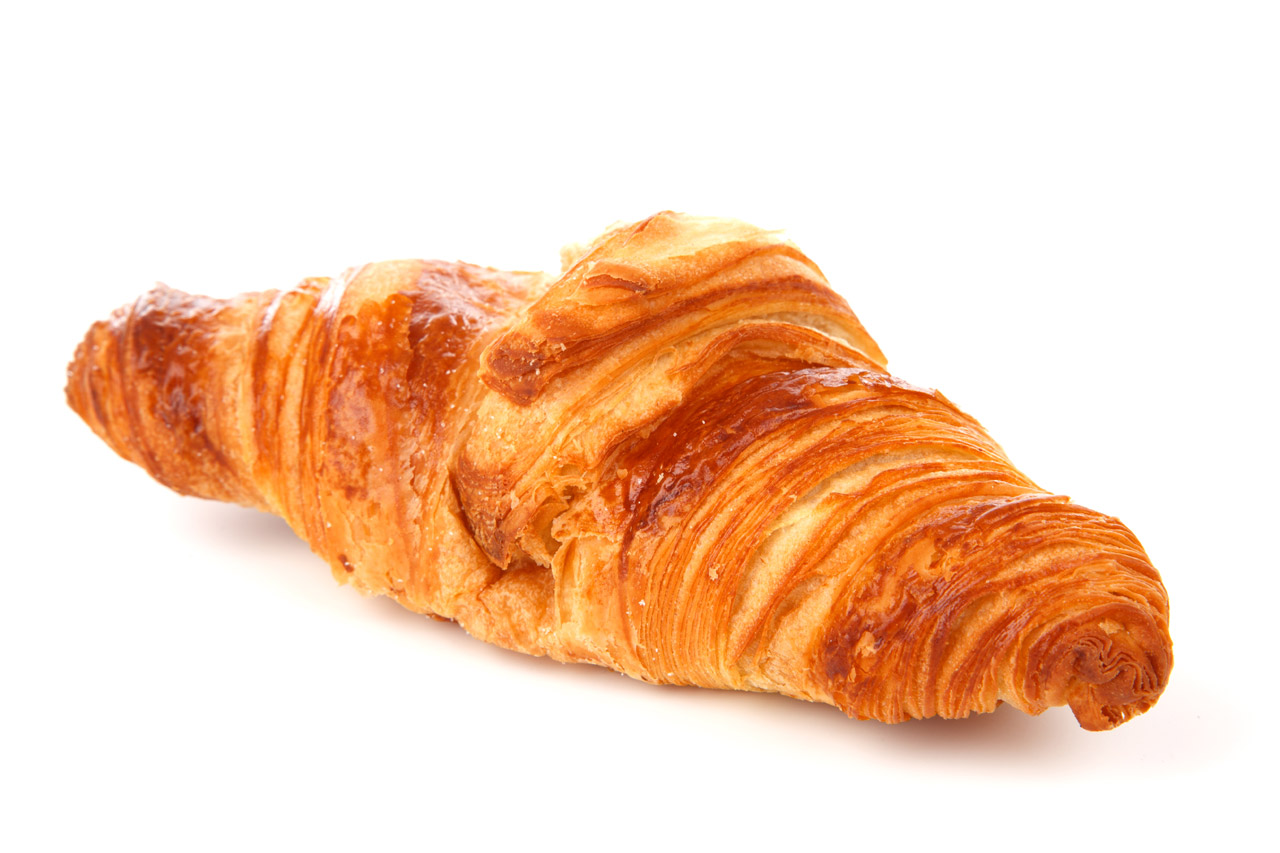
\includegraphics[width=0.31\textwidth]{figures/experiments/phase8_source.jpg}}\hfill
\subfloat[Condition A.]{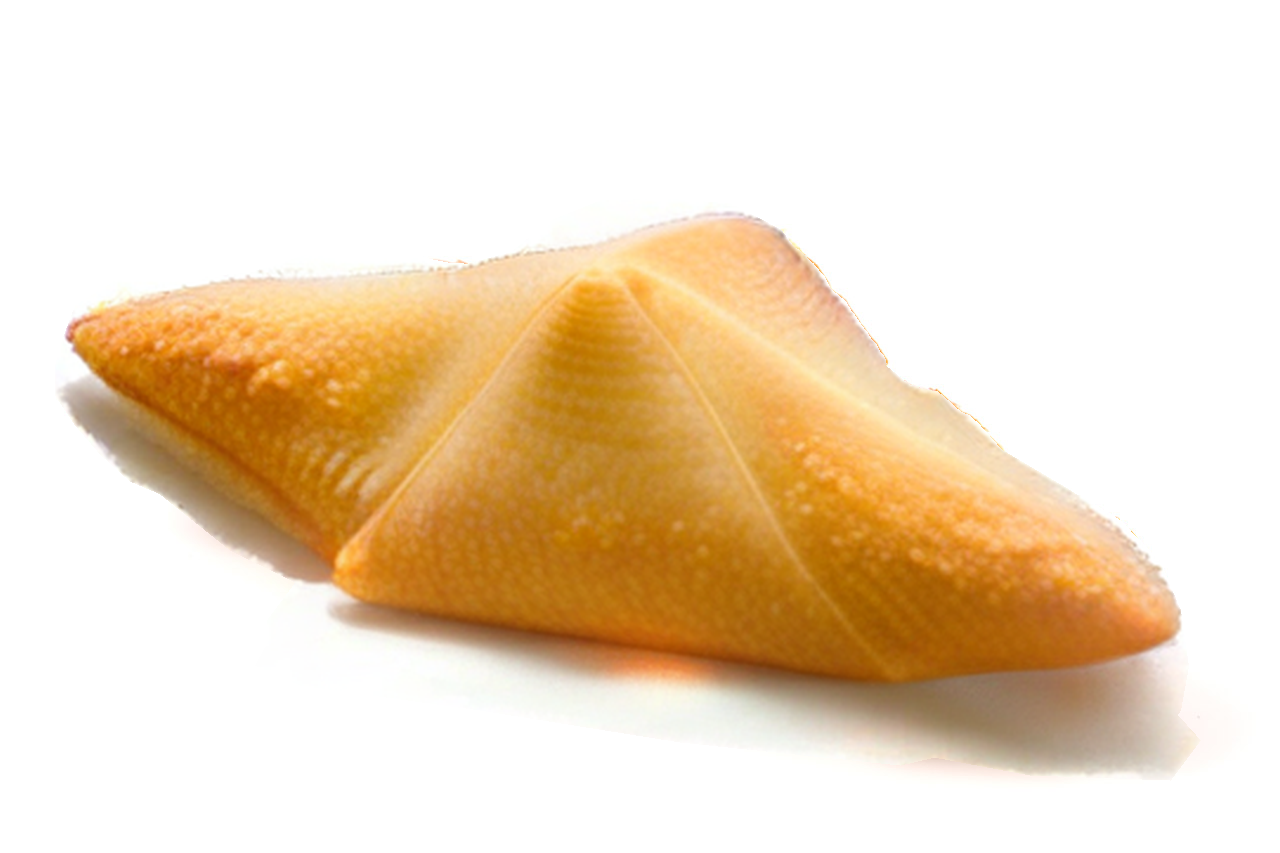
\includegraphics[width=0.31\textwidth]{figures/experiments/phase8_A.png}}\hfill
\subfloat[Condition B.]{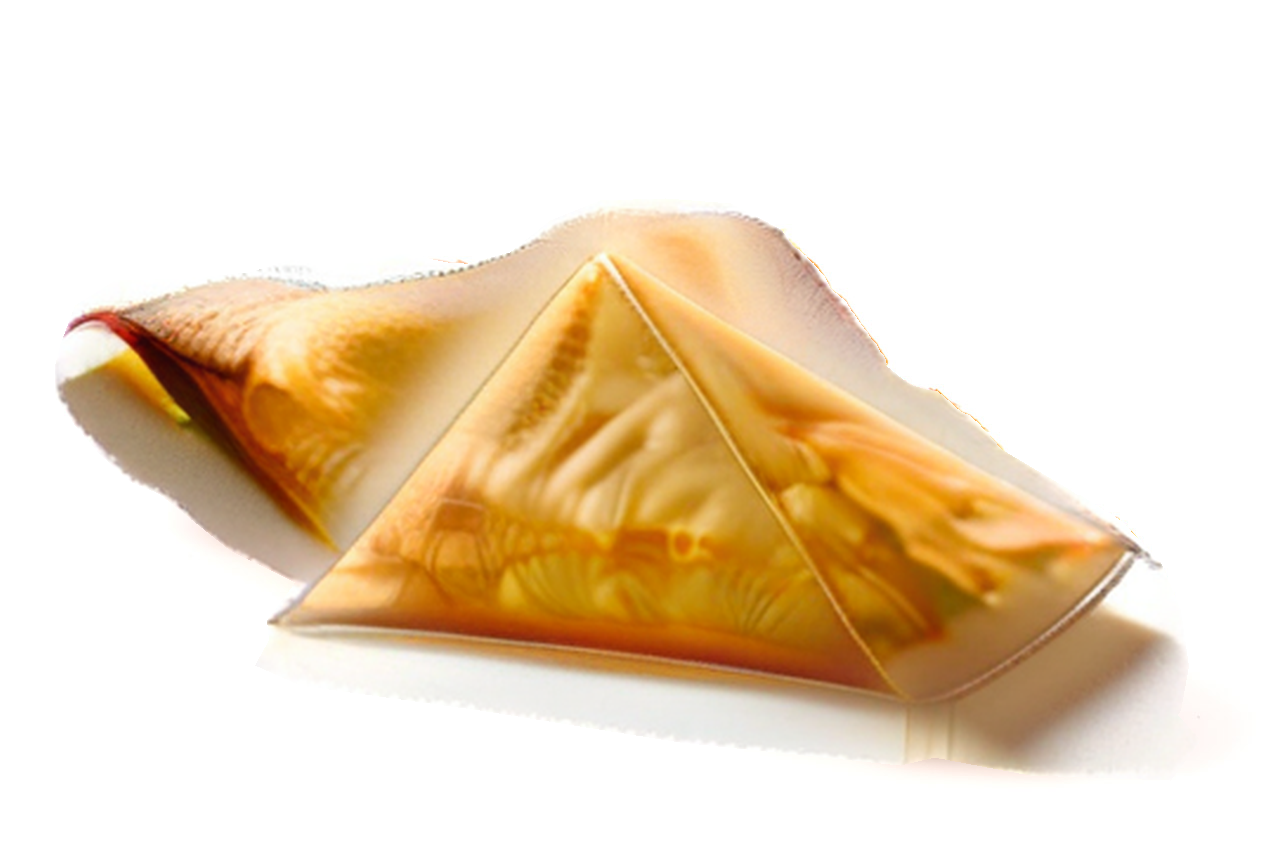
\includegraphics[width=0.31\textwidth]{figures/experiments/phase8_B.png}}
\caption[Phase 8 SDXL+Canny comparison]{Recorded Phase 8 source and two bounded SDXL+Canny conditions. The figure is evidence of an executed attempt, not a success claim.}
\label{fig:phase8}
\end{figure*}

\textbf{Analysis.} Both outputs satisfy the technical locality check. Direct user feedback on the former seed-43 result rated realism 2/5 and identified missing depth, weak texture, partial background preservation and extra food. The later A condition improved apparent volume but retained ambiguity; B regressed visually. The experiment demonstrates bounded execution, not convincing food transcreation.

\section{Experiment 3: six-case reference-guided repeatability pilot}
\textbf{Objective.} Determine whether the technically successful samosa compositing procedure can be repeated across foods, headwear and drinkware.

\textbf{Experimental setup.} Six frozen cases use isolated studio photographs from Wikimedia Commons. CASE\_01 is a historical croissant-to-samosa baseline; CASE\_02--06 are new runs. Dependent measurements are changes within and outside permitted masks, protected differences, residual source pixels and deterministic replay.

\begin{table*}[htbp]
\centering\small
\caption{Selected Phase 9 outputs verified from saved files. Zero outside/protected differences are exact RGB-pixel checks.}
\label{tab:pilot}
\begin{tabularx}{\textwidth}{lYrrrl}
\toprule
Case & Direction & Changed inside & Outside / protected & Replay & Human status\\
\midrule
01 & French $\rightarrow$ Indian & 469,215 & 0 / 0 & Yes & Historical pass\\
02 & German $\rightarrow$ French & 2,499,350 & 0 / 0 & Yes & Pending\\
03 & American $\rightarrow$ Japanese & 2,404,354 & 0 / 0 & Yes & Pending\\
04 & Italian $\rightarrow$ Moroccan & 2,367,722 & 0 / 0 & Yes & Pending\\
05 & Moroccan $\rightarrow$ Italian & 11,815,546 & 0 / 0 & Yes & Pending\\
06 & Western $\rightarrow$ Japanese & 1,298,848 & 0 / 0 & Yes & Pending\\
\bottomrule
\end{tabularx}
\end{table*}

\begin{figure*}[htbp]
\centering
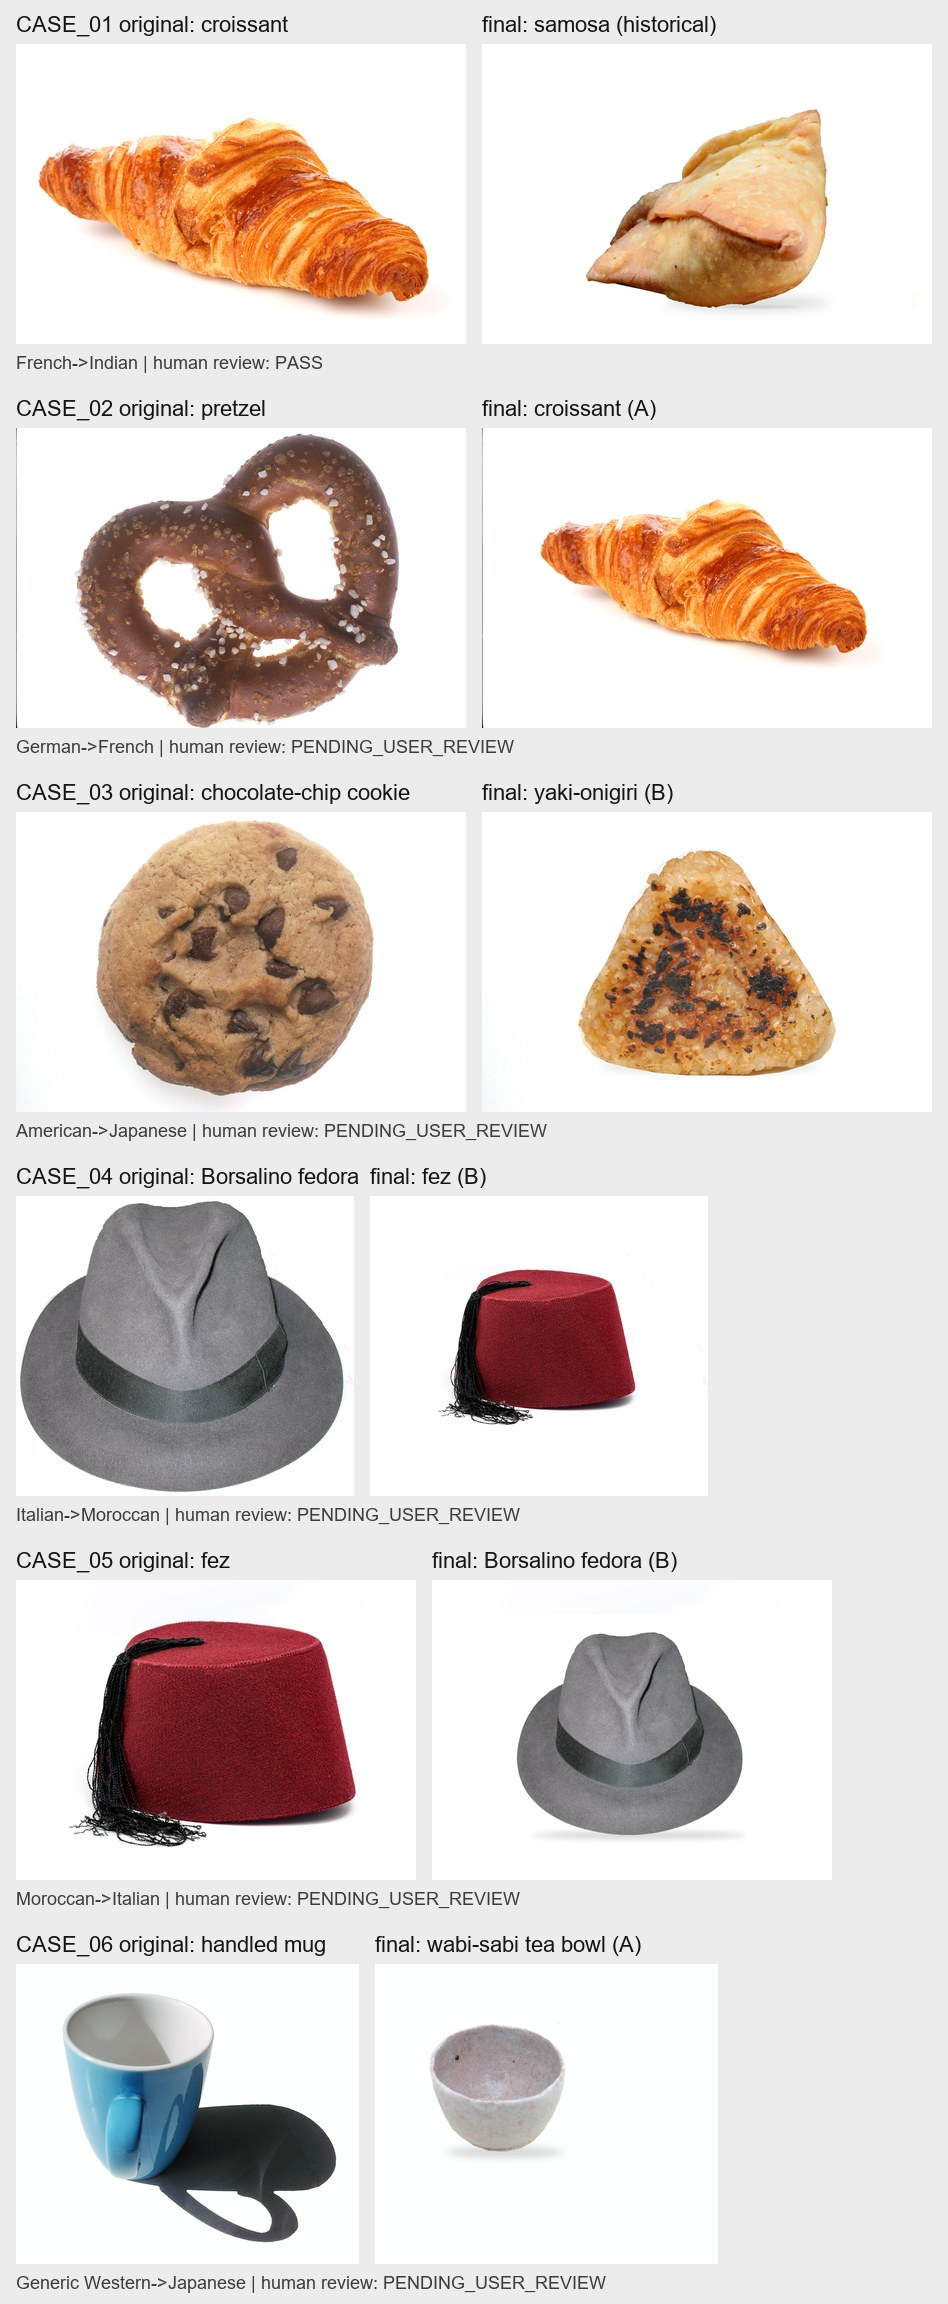
\includegraphics[width=0.94\textwidth,height=0.62\textheight,keepaspectratio]{figures/experiments/phase9_overview.jpg}
\caption{Six-case Phase 9 pilot overview. All cases are technically verified; visual reviews remain pending except the historical first case.}
\label{fig:pilot-overview}
\end{figure*}

\begin{figure*}[htbp]
\centering
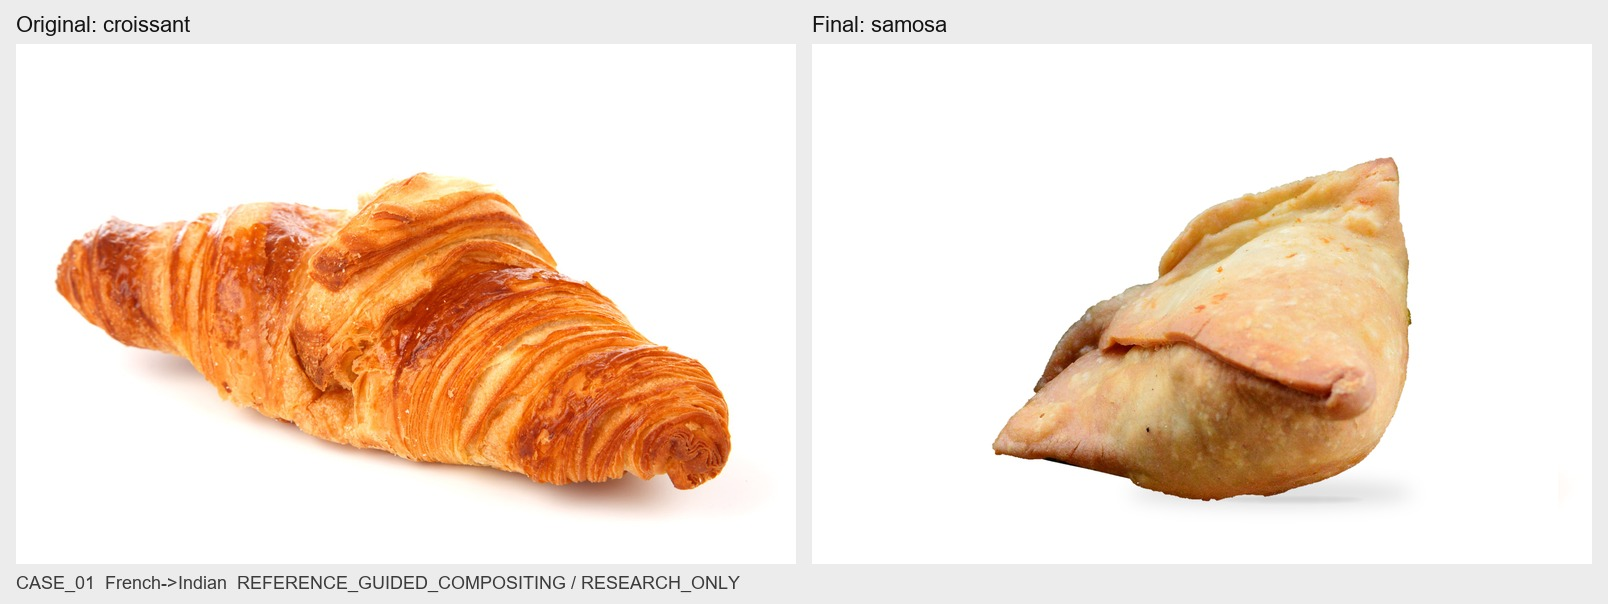
\includegraphics[width=0.94\textwidth]{figures/experiments/case01_comparison.jpg}
\caption{Historical CASE\_01: croissant to samosa. This is the only selected pilot case with a direct user pass.}
\label{fig:case01}
\end{figure*}

\begin{figure*}[htbp]
\centering
\begin{tikzpicture}
\begin{axis}[width=0.92\textwidth,height=7cm,ybar,bar width=11pt,ylabel={Changed pixels (millions)},xlabel={Selected case},symbolic x coords={02,03,04,05,06},xtick=data,ymajorgrids=true,grid style=dashed,ymin=0,legend style={at={(0.5,-0.22)},anchor=north,legend columns=2}]
\addplot+[fill=blue!60] table[x=case,y=changed_inside_millions,col sep=comma]{experiments/results/phase9_selected.csv};
\addplot+[fill=orange!80] table[x=case,y=permitted_millions,col sep=comma]{experiments/results/phase9_selected.csv};
\legend{Changed inside permitted region,Permitted region}
\end{axis}
\end{tikzpicture}
\caption[Phase 9 selected-attempt pixels]{Actual selected-attempt pixel counts from Phase 9. The changed-pixel count is at or below the permitted-region size; zero exterior changes are reported in \cref{tab:pilot}.}
\label{fig:pilot-pixels}
\end{figure*}

\textbf{Results.} The verifier reported PASS for six cases, 75 recorded files with no missing or tampered file, zero outside-region changes and zero protected differences. All selected attempts replayed identically. Four of the five new cases were labelled \emph{partial} by the assistant due to patch edges, lighting mismatch, detached shadows or low-resolution reference material. These observations must not be interpreted as human scores.

\textbf{Limitations.} The cases are a convenience sample of clean, near-white studio photos; several inputs or references are reused. The metric verifies containment rather than quality. One historical user pass is not an independent panel, and five new cases lack a human decision. Therefore the pilot supports technical repeatability only.

\section{Supplementary guided full-scene illustration}
\begin{figure*}[htbp]
\centering
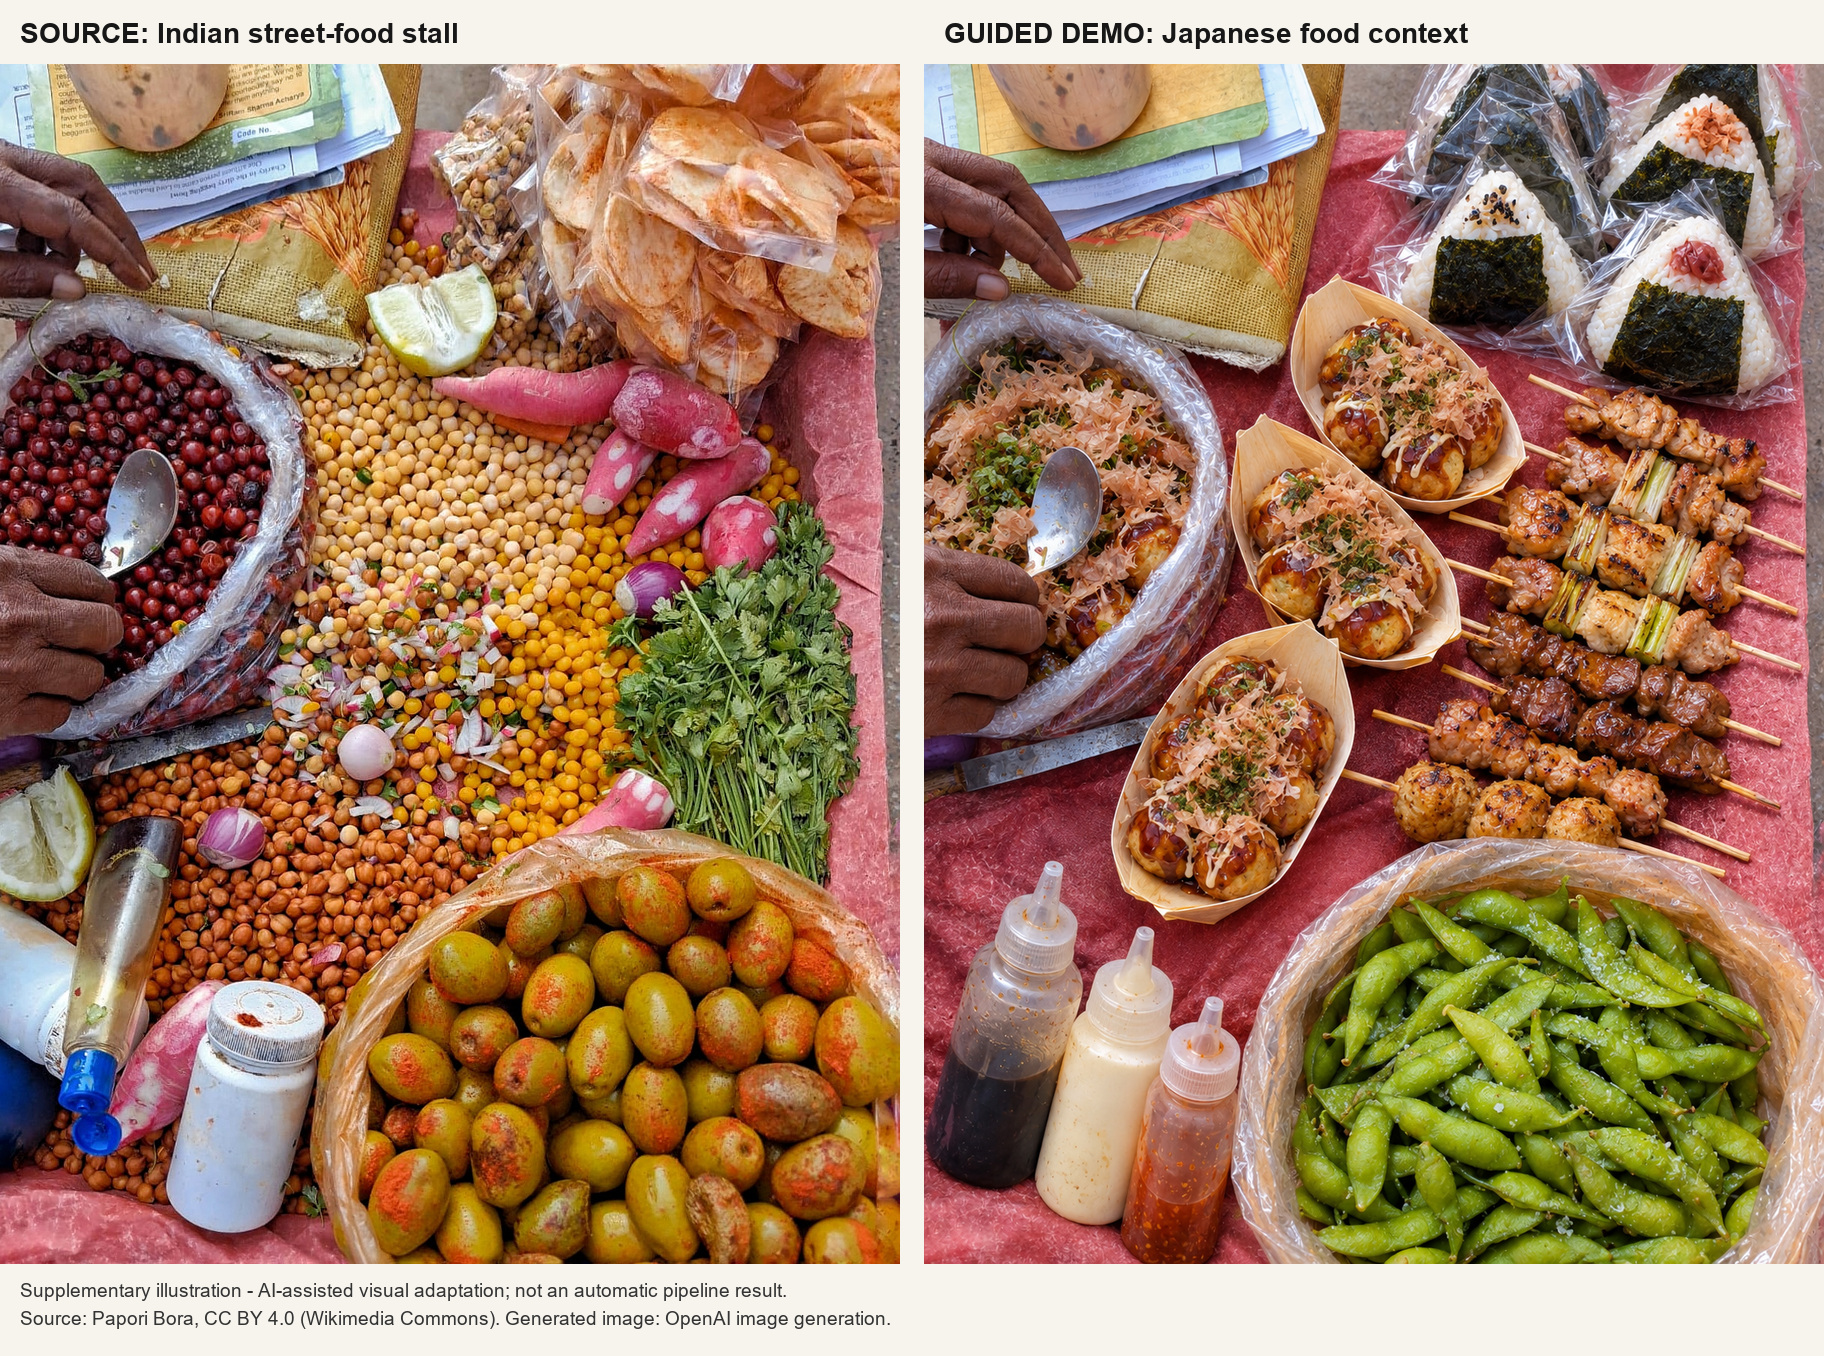
\includegraphics[width=0.95\textwidth,height=0.62\textheight,keepaspectratio]{figures/submission_demo/guided_full_scene_demo.jpg}
\caption{Supplementary guided India-to-Japan food-context illustration. It is visually useful for explaining the concept but is excluded from all experimental tables because it was produced by an external AI image editor, not the validated project pipeline. Source attribution and licence are supplied in the accompanying repository note.}
\label{fig:guided-demo}
\end{figure*}
